\chapter{Disparity Map Estimation}
\label{sec:DisparityMapEstimation}

This chapter introduces the tools available in OTB for the estimation
of geometric disparities between images.


\section{Disparity Maps}
\ifitkFullVersion
\label{sec:DisparityMaps}
\fi

The problem we want to deal with is the one of the
automatic disparity map estimation of images acquired with different sensors. By different
sensors, we mean sensors which produce images with different
radiometric properties, that is, sensors which measure different
physical magnitudes: optical sensors operating in different spectral
bands, radar and optical sensors, etc.\\

For this kind of image pairs, the classical approach of fine
correlation \cite{correl1,correl2}, can not always be used to
provide the required accuracy, since this similarity measure (the correlation
coefficient) can only measure similarities up to an affine
transformation of the radiometries.\\

There are two main questions which can be asked about what we want to
do:
\begin{enumerate}
\item Can we define what the similarity is between, for instance, a radar
and an optical image?
\item What does {\em fine registration} mean in the case where the
geometric distortions are so big and the source of information can be
located in different places (for instance, the same edge can be
produced by the edge of the roof of a building in an optical image and
by the wall-ground bounce in a radar image)?
\end{enumerate}

We can answer by saying that the images of the same object obtained by different
sensors are two different representations of the same reality. For the
same spatial location, we have two different measures. Both informations
come from the same source and thus they have a lot of common
information. This relationship may not be perfect, but it can be
evaluated in a relative way: different geometrical distortions are
compared and the one leading to the strongest link between the two
measures is kept.\\

%% proposed by Ventura et al. \cite{ventura}. They even applied it to the
%% problem of image to map registration. The approach was also finding HP
%% by matching extracted features.\\


%% Dai and Khorram \cite{xiaolong} use a feature based approach: they
%% extract closed edges which are characterized using invariant
%% moments. Then, the extracted areas are matched using their
%% characterization. Finally, the centers of gravity of each area are
%% used as HP for the estimation of an affine transformation. They apply
%% the approach to Landsat images and they obtain an accuracy better than
%% one pixel, which is similar to the accuracy obtained with manual registration.\\

%% Djamdji et al. \cite{djamdji} propose a multiresolution approach where
%% the discrete wavelet transform is used. The automatic extraction of
%% HP is done by comparing thresholded wavelet coefficients.\\

%% All these approaches try to extract HP in order to
%% compute an analytical deformation model. On the other hand,
When
working with images acquired with the same (type of) sensor one can
use a very effective approach. Since a correlation coefficient measure
is robust and fast for similar images, one can afford to apply it in
every pixel of one image in order to search for the corresponding
HP in the other image. One can thus build a deformation
grid (a sampling of the deformation map). If the sampling step of this grid is short enough, the
interpolation using an analytical model is not needed and high
frequency deformations can be estimated. The obtained grid can be used
as a re-sampling grid and thus obtain the registered images.\\

No doubt, this approach, combined with image interpolation techniques
(in order to estimate sub-pixel deformations) and multi-resolution
strategies allows for obtaining the best performances in terms of
deformation estimation, and hence for the automatic image
registration.\\

Unfortunately, in the multi-sensor case, the correlation coefficient
can not be used. We will thus try to find similarity measures which can be
applied in the multi-sensor case with the same approach as the
correlation coefficient.\\

%% \section{Model for the image registration problem\label{model}}
%% In this section,
We start by giving several definitions which allow for the
formalization of the image registration problem. First of all, we
define the master image and the slave image:
\begin{defin}
Master image: image to which other images will be registered; its
geometry is considered as the reference.
\end{defin}

\begin{defin}
Slave image: image to be geometrically transformed in order to be
registered to the master image.
\end{defin}

Two main concepts are the one of {\em similarity measure} and the one
of {\em geometric transformation}:
\begin{defin}
\label{def-simil}Let $I$ and $J$ be two images and let $c$ a similarity
criterion, we call similarity measure any scalar, strictly positive function 
\begin{equation}
S_c(I,J) = f(I,J,c).
\end{equation}

$S_c$ has an absolute maximum when the two images $I$ and $J$
are {\it identical} in the sense of the criterion $c$.\\
\end{defin}

\begin{defin}\label{defin-T}
A geometric transformation $T$ is an operator which, applied to the
coordinates $(x,y)$ of a point in the slave image, gives the
coordinates $(u,v)$ of its HP in the master image:

\begin{equation}
\left( \begin{array}{c}
u\\
v\\
\end{array}\right) = T \left( \begin{array}{c}
x\\
y\\
\end{array}\right)
\label{Tgeom}
\end{equation}

\end{defin}

Finally we introduce a definition for the image registration problem:
\begin{defin}\label{defin-recal}
Registration problem: \begin{enumerate}
\item determine a geometric transformation $T$ which maximizes the
similarity between a master image $I$ and the result of the
transformation $T\circ J$:
\begin{equation}
Arg \max_T(S_c(I,T\circ J));
\end{equation}
\item re-sampling of $J$ by applying $T$.
\end{enumerate}

\end{defin}

%% We must note that Le Moigne et al. have proposed in a recent contribution
%% \cite{ig02lemoigne} a modular approach for the
%% registration which allows the analysis of different similarity
%% measures and different optimization strategies. The presented results,
%% which are still preliminary, are very promising. The multi-sensor
%% case has been dealt with, but only for optical images (Ikonos and
%% Landsat/ETM+). The case of very different images (for instance optical
%% and radar) has not been explored.\\


\subsection{Geometric deformation modeling\label{sec-model}}
The geometric transformation of definition \ref{defin-T} is used for
the correction of the existing deformation between the two images to be
registered. This deformation contains informations which are linked to
the observed scene and the acquisition conditions. They
can be classified into 3 classes depending on their physical source:
\begin{enumerate}
\item deformations linked to the mean attitude of the sensor
(incidence angle, presence or absence of yaw steering, etc.);
\item deformations linked to a stereo vision (mainly due to the topography);
\item deformations linked to attitude evolution during the acquisition
(vibrations which are mainly present in push-broom sensors).
\end{enumerate}

These deformations are characterized by their spatial frequencies and
intensities which are summarized in table \ref{tab-deform}.\\

\begin{table}[b]
\begin{center}
\begin{tabular}{|c|c|c|}
\hline
& Intensity & Spatial Frequency\\
\hline
Mean Attitude & Strong & Low \\
\hline
Stereo & Medium & High and Medium\\
\hline
Attitude evolution & Low & Low to Medium \\
\hline
\end{tabular}
\end{center}
\caption{Characterization of the geometric deformation sources}
\label{tab-deform}
\end{table}

Depending on the type of deformation to be corrected, its model will be
different. For example, if the only deformation to be corrected is the
one introduced by the mean attitude, a physical model for the
acquisition geometry (independent of the image contents) will be
enough. If the sensor is not well known, this deformation can be
approximated by a simple analytical model. When the deformations to be
modeled are high frequency, analytical (parametric) models are not
suitable for a fine registration. In this case, one has to use a fine
sampling of the deformation, that means the use of deformation
grids. These grids give, for a set of pixels of the master image,
their location in the slave image.\\

The following points summarize the problem of the deformation modeling:
\begin{enumerate}
\item An analytical model is just an approximation of the
deformation. It is often obtained as follows:
\begin{enumerate}
\item Directly from a physical model without using any image content information.
\item By estimation of the parameters of an a priori model
(polynomial, affine, etc.). These parameters can be estimated:
\begin{enumerate}
\item Either by solving the equations obtained by taking HP. The HP can be manually or automatically extracted.
\item Or by maximization of a global similarity measure.
\end{enumerate}

\end{enumerate}
\item A deformation grid is a sampling of the deformation map.
\end{enumerate}

The last point implies that the sampling period of the grid must be short
enough in order to account for high frequency deformations (Shannon
theorem). Of course, if the deformations are non stationary (it is
usually the case of topographic deformations), the sampling can 
be irregular.\\

As a conclusion, we can say that definition \ref{defin-recal} poses
the registration problem as an optimization problem. This optimization
can be either global or local with a similarity measure which can also
be either local or global. All this is synthesized in table  \ref{tab-approches}.\\

\begin{table}[b]
\begin{center}
\begin{tabular}{|c|c|c|}
\hline
Geometric model & Similarity measure & Optimization of the \\
& & deformation \\
\hline
Physical model & None & Global \\
\hline
Analytical model  & Local & Global \\
with a priori HP & & \\
\hline
Analytical model& Global & Global \\
without a priori HP & & \\
\hline
Grid & Local & Local \\
\hline
\end{tabular}
\end{center}
\caption{Approaches to image registration}
\label{tab-approches}
\end{table}

The ideal approach would consist in a registration which is locally
optimized, both in similarity and deformation, in order to have the
best registration quality. This is the case when deformation grids with
dense sampling are used. Unfortunately, this case is the most
computationally heavy and one often uses either a low sampling rate of
the grid, or the evaluation of the similarity in a small set of pixels
for the estimation of an analytical model. Both of these choices lead to local registration
errors which, depending on the topography, can amount several
pixels.\\

Even if this registration accuracy can be enough in many
applications, (ortho-registration, import into a GIS, etc.), it is not
acceptable in the case of data fusion, multi-channel segmentation or
change detection \cite{townshend}. This is why we will focus on the
problem of deformation estimation using dense grids.\\

%% None of the references presented in section \ref{review} uses the
%% local optimization approach. We can also note that in the multi-sensor
%% case only few authors \cite{ig02lemoigne} have used any similarity
%% measure other than the correlation coefficient. However, in the
%% medical imaging field, as we will see in section \ref{sec-simil}, a
%% lot of similarity measures have been proposed as a generalization of
%% the correlation coefficient. These measures enable the registration of
%% very different imagery modalities. Nevertheless, these works are not
%% directly usable in our problem since the geometric deformations
%% present in medical images can be easily represented by global
%% analytical models. Indeed, often a rigid model (rotation, translation,
%% scale) or slightly elastic (affine plus a $a\cdot x\cdot y$ term) is
%% enough since the sensors are stable, the stereo effect is small and
%% only the point of view changes. As we have noted above, deformations
%% due to topography can locally have high frequencies for medium and
%% high resolution sensors (30 m. and better), thus our need for a fine
%% modeling. We also point out that the problem of hidden faces is beyond
%% the scope of this paper.\\


\subsection{Similarity measures\label{sec-simil}}


The fine modeling of the geometric deformation we are looking for
needs for the estimation of the coordinates of nearly every pixel in
the master image inside the slave image. In the classical mono-sensor
case where we use the correlation coefficient we proceed as follows.\\

The geometric deformation is modeled by local rigid displacements. One
wants to estimate the coordinates of each pixel of the master image inside the
slave image. This can be represented by a displacement vector
associated to every pixel of the master image. Each of the two components
(lines and columns) of this vector field will be called deformation grid.\\

We use a small window taken in the master image and we test the similarity
for every possible shift within an exploration area inside the slave
image (figure \ref{zones}). \\

\begin{figure}
%\begin{center}{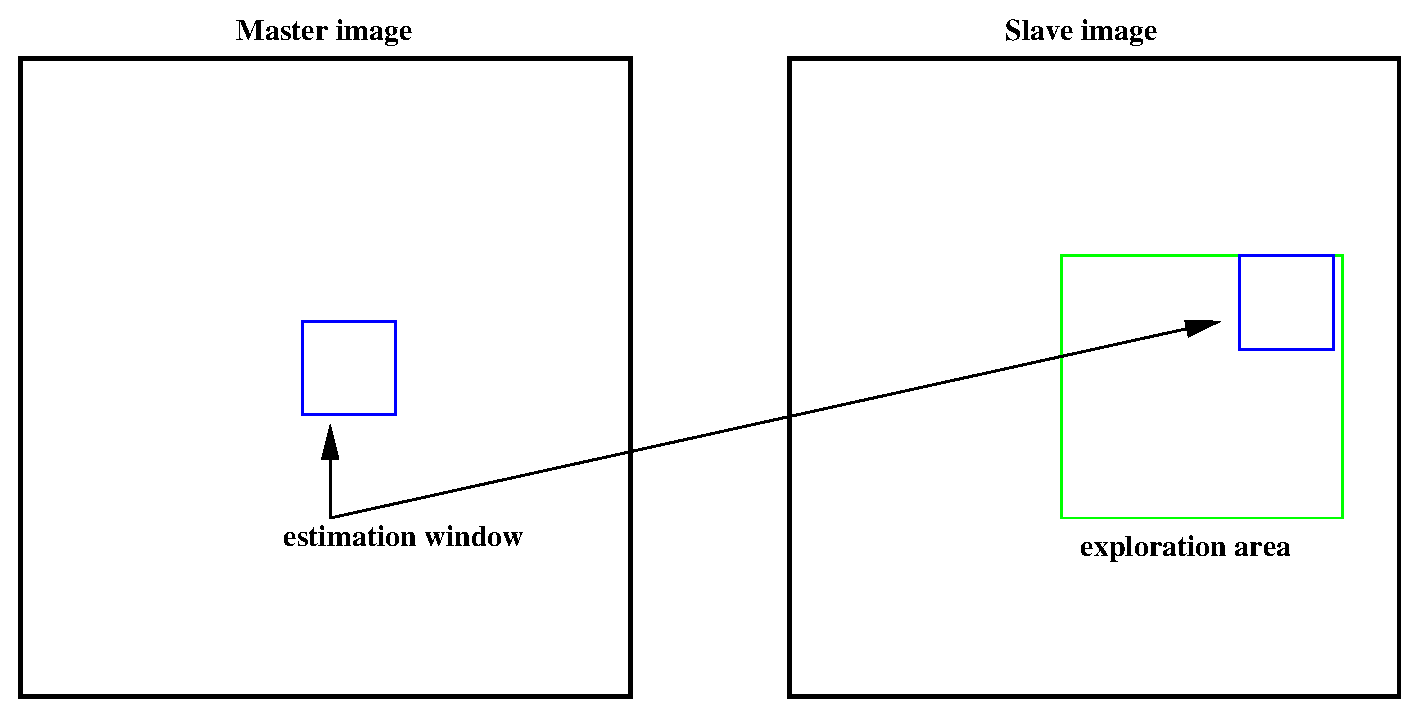
\includegraphics[width=0.8\hsize]{zones.eps}}
  \begin{center}
    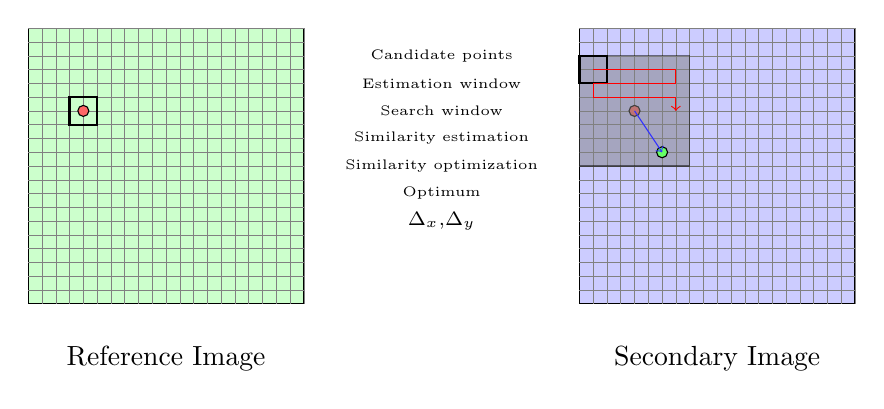
\begin{tikzpicture}[scale=0.35]
    \draw[fill=green!20] (5,5) rectangle (15,15);
    \draw[step=0.5, gray, very thin] (5,5) grid (15,15);
    \node (Reference) at (10,3) {Reference Image};

    \draw[fill=blue!20] (25,5) rectangle (35,15);
    \draw[step=0.5, gray, very thin] (25,5) grid (35,15);
    \node (Reference) at (30,3) {Secondary Image};
    
    \draw[fill=red!60] (7,12) circle (0.2);
    \draw[fill=red!60] (27,12) circle (0.2);
    \node (CPs) at (20,14) {\tiny Candidate points};
    
    \draw[thick] (6.5,11.5) rectangle +(1,1);
    \node (EW) at (20,13) {\tiny Estimation window};
    
    \draw[fill=gray, opacity=0.5] (25,10) rectangle +(4,4);
    \node (SW) at (20,12) {\tiny Search window};
    
    \draw[thick] (25,13) rectangle +(1,1);
    \node (SEW) at (20,11) {\tiny Similarity estimation};
    
    \draw[red,->] (25.5,13.5) --  ++(3,0) -- ++(0,-0.5) -- ++(-3,0) -- ++(0,-0.5) --++(3,0) -- ++(0,-0.5)  ;
    \node (OPT) at (20,10) {\tiny Similarity optimization};
    
    \draw[fill=green!60] (28,10.5) circle (0.2);
    \node (OPTF) at (20,9) {\tiny Optimum};
    
    \draw[blue!80,->] (27,12) -- (28,10.5);
    \node (Deltas) at (20,8) {$\scriptstyle{\Delta_x,\Delta_y}$};
    
  \end{tikzpicture}
    \end{center}
\caption{Estimation of the correlation surface.}
\label{zones}
\end{figure}


That means that for each position we compute the correlation
coefficient. The result is a correlation surface whose
maximum gives the most likely local shift between both images:

\begin{equation}
\begin{split}
&\rho_{I,J}(\Delta x, \Delta y) = \\
&\frac{1}{N}\frac{\sum_{x,y}(I(x,y)-m_I)(J(x+\Delta x,y+\Delta y)-m_J)}{\sigma_I
\sigma_J}.
\end{split}
\end{equation}

In this expression, $N$ is the number of pixels of the analysis
window, $m_I$ and $m_J$ are the estimated mean values inside the
analysis window of respectively image $I$ and image $J$ and $\sigma_I$
and $\sigma_J$ are their standard deviations.\\

Quality criteria can be applied to the estimated maximum in order to
 give a confidence factor to the estimated shift: width of the peak,
 maximum value, etc. Sub-pixel shifts can be measured by applying
 fractional shifts to the sliding window. This can be done by image interpolation.\\

The interesting parameters of the procedure are:
\begin{itemize}
\item The size of the exploration area: it determines the
computational load of the algorithm (we want to reduce it), but it has
to be large enough in order to cope with large deformations.
\item The size of the sliding window: the robustness of the correlation
coefficient estimation increases with the window size, but the
hypothesis of local rigid shifts may not be valid for large windows.
\end{itemize}

The correlation coefficient cannot be used with original grey-level
images in the multi-sensor case. It could be used on extracted
features (edges, etc.), but the feature extraction can introduce
localization errors. Also, when the images come from sensors using
very different modalities, it can be difficult to find similar
features in both images. In this case, one can try to find the
similarity at the pixel level, but with other similarity measures and
apply the same approach as we have just described.\\

The concept of similarity measure has been presented in definition
\ref{def-simil}. The difficulty of the procedure lies in finding the
function $f$ which properly represents the criterion $c$. We also need
that $f$ be easily and robustly estimated with small windows. We extend here what we proposed in \cite{ig02simil}.\\

\subsection{The correlation coefficient\label{expe}}
We remind here the computation of the correlation coefficient between
two image windows $I$ and $J$. The coordinates of the pixels inside
the windows are represented by $(x,y)$:

\begin{equation}
\rho(I,J) = \frac{1}{N}\frac{\sum_{x,y}(I(x,y)-m_I)(J(x,y)-m_J)}{\sigma_I
\sigma_J}.
\label{coeffcorr}
\end{equation}

In order to qualitatively characterize the different similarity
measures we propose the following experiment. We take two images which
are perfectly registered and we extract a small window
of size $N\times M$ from each of the images (this size is set to
$101\times 101$ for this experiment). For the master image, the
window will be centered on coordinates $(x_0,
y_0)$ (the center of the image) and for the slave image, it will be centered on coordinates $(x_0+\Delta x,
y_0)$. With different values of $\Delta x$ (from -10 pixels to 10
pixels in our experiments), we obtain an estimate of $\rho(I,J)$ as a
function of $\Delta x$, which we write as
$\rho(\Delta x)$ for short. The obtained curve should have a maximum for
$\Delta x =0$, since the images are perfectly registered. We would
also like to have an absolute maximum with a high value and with a
sharp peak, in order to have a good precision for the shift estimate.\\

%% In the following, we will make this experiment with different image
%% pairs and different similarity measures. Figure \ref{fig-correl}
%% shows the results obtained when the correlation coefficient is applied
%%  to (\ref{correl-B1B1}) one extract of the B1 channel of a Spot 5
%% image with itself, (\ref{correl-B1B3}) an extract of channel B1 with the
%% extract of channel B3,  and (\ref{correl-B1ERS}) the extract of
%% channel B1 with an
%% extract of an ERS-2 SAR image. The images are presented in figures
%% \ref{histo_b1_b1}, \ref{histo_b1_b3} and \ref{histo_b1_ers}.\\


%% % \begin{figure*}
%% % \centerline{\subfigure[Correlation B1-B1]{\includegraphics[width=0.5\hsize]{CORREL_b1_b1_10.pdf}\label{correl-B1B1}} \\
%% % \subfigure[Correlation
%% % B1-B3]{\includegraphics[width=0.5\hsize]{CORREL_b1_b3_10.pdf}\label{correl-B1B3}}\\
%% % \subfigure[Correlation B1-ERS]{\includegraphics[width=0.5\hsize]{CORREL_b1_ERS_10_0.pdf}\label{correl-B1ERS}}}
%% % \caption{Measure of $\rho(\Delta x)$ for 3 different pairs of images.}
%% % \label{fig-correl}
%% % \end{figure*}

%% \begin{figure*}
%% \centering
%% \subfigure[Correlation B1-B1]{\includegraphics[width=0.4\hsize]{CORREL_b1_b1_10.pdf}\label{correl-B1B1}} \\
%% \subfigure[Correlation
%% B1-B3]{\includegraphics[width=0.4\hsize]{CORREL_b1_b3_10.pdf}\label{correl-B1B3}}\\
%% \subfigure[Correlation B1-ERS]{\includegraphics[width=0.4\hsize]{CORREL_b1_ERS_10_0.pdf}\label{correl-B1ERS}}
%% \caption{Measure of $\rho(\Delta x)$ for 3 different pairs of images.}
%% \label{fig-correl}
%% \end{figure*}

%% We can see that the correlation coefficient has a good behavior for
%% the first pair, but its performances are bad when the images
%% radiometries are different. The correlation coefficient
%%  can be characterized as follows:
%% \begin{itemize}
%% \item Well known algorithm.
%% \item Fits the registration needs when using radiometrically similar images.
%% \item Simple and fast computation.
%% \item High precision in the estimation of the deformation.
%% \item Robust to noise.
%% \end{itemize}

%% However its main disadvantage is that it can only take into account
%%  affine transformations between radiometries ($j = \alpha i + \beta$)
%%  so it can not be used in the general multi-sensor case.\\


%% \subsection{Generalization: probabilistic interpretation \label{sec_correl}}
%% The correlation coefficient formulation (equation \ref{coeffcorr}) can
%% be revisited with a probabilistic interpretation:

%% \begin{equation}
%% \begin{split}
%% \rho(I,J) &= \frac{1}{N}\frac{\sum_{x,y}(I(x,y)-m_I)(J(x,y)-m_J)}{\sigma_I
%% \sigma_J} \\
%% &= \sum_{(i,j)}\frac{(i-m_I)(j-m_J)}{\sigma_I \sigma_J}p_{ij}
%% \end{split}
%% \label{coeffcorr2}
%% \end{equation}

%% where the sum is taken over the list of radiometry pairs $(i,j)$, and
%% $p_{ij}$ is the value of the joint normalized histogram (estimation of
%% the joint probability density function, pdf, $f_{ij}(i,j)$) of the pair of images.\\

%% That means that we are assuming a linear model
%% \begin{equation}
%% j = (i-m_I)\frac{\sigma_J}{\sigma_I}+m_J,
%% \end{equation}
%% and we evaluate its likelihood by weighting with the probability of
%% each radiometry couple, $p_{ij}$.\\

%% One could assume different models for the radiometry pairs leading to
%% different measures as, for instance, the identity model , $i=j$, which
%% leads to the $L_n$ norm:

%% \begin{equation}
%% L_n(I,J) = \sum_{i,j} \left| i - j\right|^n p_{ij},
%% \end{equation}

%% or more complex models based on textural approaches :

%% Diagonal moment:
%% \begin{equation}
%% MD(I,J) = \sum_{i,j}\left| i - j\right|(i+j-\sigma_I-\sigma_J) p_{ij},
%% \end{equation}

%%  Cluster Shade:
%% \begin{equation}
%% C_{shade}(I,J) = \sum_{i,j} (i+j-\sigma_I-\sigma_J)^3 p_{ij},
%% \end{equation}

%%  Cluster Prominence:
%% \begin{equation}
%% C_{pro}(I,J) = \sum_{i,j} (i+j-\sigma_I-\sigma_J)^4 p_{ij}.
%% \end{equation}

%% An assessment of these measures for image registration can be found in
%% \cite{bro}. They are very sensitive to noise and are not useful for
%% the comparison of grey-levels of multi-sensor image pairs.\\

%% \subsection{Estimation of similarity measures and $p_{IJ}$}

%% In the expression of the correlation coefficient the term $p_{ij}$ is
%% an estimation of the joint pdf of the radiometries of
%% the images we are comparing. It can be seen as a link (transfer
%% function) between both radiometries.\\

%% % We want a measure of the
%% % similarity measure which is valid locally, that is, which takes into
%% % account the specificities of the neighborhood of the pixel for which
%% % we are estimating the deformation. That means that we have to use a
%% % small estimation window around the pixel of interest. On the other
%% % hand, we want a robust estimate, thus we need reliable values of
%% % $p_{ij}$, which means the use of a high number of samples.\\


%% %\subsubsection{Examples of $p_{ij}$ estimation}

%% We show here several examples of the estimation of the joint
%% histogram. On figures \ref{histo_b1_b1}, \ref{histo_b1_b3} and
%% \ref{histo_b1_ers} are shown respectively the joint histograms of one
%% image with itself (B1-B1), two different channels of the same Spot 5
%% image (B1-B3) and a Spot 5 B3 - ERS-2 pair.\\

%% \begin{figure}
%% \centering
%% \subfigure[SPOT 5 B1]{\includegraphics[width=0.5\hsize]{b1_1980_1980.pdf}} \\
%% \subfigure[Joint histogram]{\includegraphics[width=0.5\hsize]{hb1.pdf}}
%% \caption{Joint histogram of an image with itself.}
%% \label{histo_b1_b1}
%% \end{figure}


%% \begin{figure}
%% \centering
%% \subfigure[SPOT 5 B1]{\includegraphics[width=0.5\hsize]{b1_3376_3882.pdf}}\\
%% \subfigure[SPOT 5 B3]{\includegraphics[width=0.5\hsize]{b3_3376_3882.pdf}}\\
%% \subfigure[Joint histogram]{\includegraphics[width=0.5\hsize]{hb3.pdf}}\\
%% \caption{Joint histogram of two channels (B1-B3) of the same Spot 5 image.}
%% \label{histo_b1_b3}
%% \end{figure}



%% \begin{figure}
%% \centering
%% \subfigure[SPOT 5 B3]{\includegraphics[width=0.5\hsize]{b1_1500_2500.pdf}}\\
%% \subfigure[ERS-2]{\includegraphics[width=0.5\hsize]{ERS_1500_2500.pdf}}\\
%% \subfigure[Joint histogram]{\includegraphics[width=0.5\hsize]{hers.pdf}}\\
%% \caption{Joint histogram of a Spot 5 B3 image and a ERS-2 image.}
%% \label{histo_b1_ers}
%% \end{figure}

%% As expected, the joint histogram of an image with itself is a straight
%% line with slope 1. It shows the full correlation between the two
%% images: the identity transfer function. This kind of situation is well
%% dealt with by the correlation coefficient.\\

%% The B1-B3 case (figure \ref{histo_b1_b3}) shows two nearly linear tendencies which are
%% mixed up. This case can not be dealt with by the correlation coefficient.\\

%% Finally, figure \ref{histo_b1_ers} shows the impossibility of finding
%% any correlation link between two sensors which are as different as an
%% optical and a radar one.\\


%% \subsubsection{Computation time}
%% The main difference between the two expressions of the correlation
%% coefficient given by equations \ref{coeffcorr} and \ref{coeffcorr2} is
%% the estimation of the joint pdf needed in the second
%% expression. This estimation is usually done by computing the joint
%% histogram. The joint histogram can be computed with different methods,
%% but their discussion is beyond the scope of this paper. However it is
%% important to note that the method chosen for histogram computation may
%% induce significative changes in the computation cost of the similarity
%% measure. As an example, with our implementation (counting with
%% optimization of the number of classes) there is an increase factor of 4 in
%% computation time between equation \ref{coeffcorr} and equation
%% \ref{coeffcorr2}.\\

%% The multi-sensor measures which will be introduced in the next section
%% need the estimation of the joint histogram. Hence, their computation
%% time is comparable to the one of equation \ref{coeffcorr2}. The
%% differences of computation complexity between these measures are
%% negligible, since the longest part of the algorithm is taken by the
%% joint histogram estimation.\\


%% \subsection{Multi-sensor measures.}
%% We introduce here several similarity measures which have been proved
%% useful in the problem of multi-modality medical image registration \cite{dsarrut-thesis}.\\

%% In the following, the sums will be computed over radiometry values. We
%% will use the conditional mean:
%% \begin{equation}
%% m_{I|j} = \frac{1}{p_j}\sum_i i p_{ij};
%% \end{equation}

%% and the conditional variance:

%% \begin{equation}
%% \sigma^2_{I|j} = \frac{1}{p_j}\sum_i (i-m_{I|j})^2 p_{ij}.
%% \end{equation}

%% For each of the following measures, we will perform the experiment
%% described in section \ref{expe}.\\


%% \subsubsection{Measures using the radiometry values and the probabilities}

%% Within this class, we will not take into account the measures which
%% are based on the differences of radiometries ($L_n$ norm of the
%% difference) \cite{tru98,cm87,akn89}, or textural measures, since they
%% give low quality results.\\


%% \paragraph{Normalised standard deviation or Woods criterion}

%% The work by Woods et al. first on mono-modal registration 
%% \cite{wcm92} and then on multi-modal registration \cite{wmc93} lead to
%% the elaboration of this similarity measure. Given the intensity on one
%% image, that is the set of pixels having this value, this measure takes
%% into account the variability of the intensities of the homologous
%% pixels in the other image. The underlying hypothesis is that this
%% variability (which is actually a measure of variance) will be minimum
%% when the images are registered:

%% \begin{equation}
%% Woods(I|J) = \sum_j \frac{\sigma_{I|j}}{m_{I|j}}p_j
%% \end{equation}

%% In order to have a criterion which has to be maximised, we will use:
%% \begin{equation}
%% S_{Woods}(I|J) = 1-\sum_j \frac{\sigma_{I|j}}{m_{I|j}}p_j
%% \end{equation}

%% The results on our three test image pairs are shown in figure
%% \ref{woods}. We see that for the mono-sensor case the results are
%% similar to those of the correlation coefficient. For the two
%% multi-sensor examples, we obtain high values near the 0-shift, but the
%% location of these maxima is not accurate.\\

%% \begin{figure*}
%% \centering
%% \subfigure[B1 with B1]{\includegraphics[width=0.4\hsize]{WOODS_b1_b1_1_60_15.pdf}}\\
%% \subfigure[B1 with B3]{\includegraphics[width=0.4\hsize]{WOODS_b1_b3_1_60_15.pdf}}\\
%% \subfigure[B1 with ERS]{\includegraphics[width=0.4\hsize]{WOODS_b1_ERS_60_15_0.pdf}}
%% \caption{Image shift experiment: Woods criterion.}
%% \label{woods}
%% \end{figure*}


%% \paragraph{Correlation ratio}

%% This is a very well known measure in statistics. It has been first
%% proposed in the framework of image registration by Roche et
%% al. \cite{rmpa98b}. It is defined as follows:
%% \begin{equation}
%% \eta^2(I|J) = 1-\frac{1}{\sigma_I^2}\sum_j \sigma_{I|j}^2p_j
%% \end{equation}

%% Its interpretation is similar to the one of the Woods criterion. The
%% results are shown in figure \ref{rapcorr} and they are worse than
%% those of the Woods criterion.\\

%% \begin{figure*}
%% \centering
%% \subfigure[B1 with B1]{\includegraphics[width=0.4\hsize]{RAPCORR_b1_b1_0_80_10.pdf}}\\
%% \subfigure[B1 with B3]{\includegraphics[width=0.4\hsize]{RAPCORR_b1_b3_1_60_10.pdf}}\\
%% \subfigure[B1 with ERS]{\includegraphics[width=0.4\hsize]{RAPCORR_b1_ERS_80_10_0.pdf}}
%% \caption{Image shift experiment: Correlation ratio.}
%% \label{rapcorr}
%% \end{figure*}

%% \subsubsection{Measures using only the probabilities}

%% This class of measures does not directly use the radiometries of the
%% pixels, but only the estimation of the joint pdf. Of course,
%% the pixel pairs are used for the estimation of this probability.\\


%% \paragraph{Distance to independence}

%% It is a normalised version of the $\chi^2$ test:
%% \begin{equation}
%% \chi^2(I,J) = \sum_{i,j}\frac{(p_{ij}-p_i p_j)^2}{p_i p_j}
%% \end{equation}

%% It measures the degree of statistical dependence between both images,
%% since for two independent random variables, the joint pdf is
%% equal to the product of the marginals. The correlation coefficient is
%% a test of independence of order 2 and this one is the generalisation
%% to any order. The results are shown in figure \ref{chi2}. In this
%% case, for the three pairs, we obtain an absolute maximum for the
%% 0-shift case which is sharp enough for a robust automatic detection.\\

%% \begin{figure*}
%% \centering
%% \subfigure[B1 with B1]{\includegraphics[width=0.4\hsize]{KI2_b1_b1_0_100_5.pdf}}\\
%% \subfigure[B1 with B3]{\includegraphics[width=0.4\hsize]{KI2_b1_b3_1_100_5.pdf}}\\
%% \subfigure[B1 with ERS]{\includegraphics[width=0.4\hsize]{KI2_b1_ERS_100_5_0.pdf}}
%% \caption{Image shift experiment: Distance to independence.}
%% \label{chi2}
%% \end{figure*}


%% \paragraph{The $f-divergence$ family}
%% A $f-divergence$ \cite{csiszar} measures the expectation of the
%% diversity of the likelihood ratio between two distributions $P$ and $Q$:

%% \begin{equation}
%% \begin{split}
%% D_{f}(P,Q) = E_Q \left[f\left( \frac{d p(x)}{d q(x)} \right)\right] 
%% =  \int f\left(\frac{p(x)}{q(x)}\right)q(x) dx
%% \end{split}
%% \end{equation}

%% $E_Q$ is the expectation with respect to $Q$, $\frac{d p(x)}{d q(x)}$
%% is the derivative with respect to a density, 
%% $f$ is continuous and convex on $[0,+\infty)$. A divergence can be
%% seen as a relative entropy. In order to simplify the
%% notation, we will use: $p=p_{ij}$, $q=p_i p_j$, $\int = \sum_{i,j}$.\\


%% \begin{table}[b]
%% \begin{center}
%% \begin{tabular}{|c|c|}
%% \hlx{hv}
%% Measure & $f(x)$ \\
%% \hlx{hv}
%% Kolmogorov distance & $\frac{1}{2}|x-1|$ \\
%% \hlx{hv}
%% Mutual information & $x\log x$ \\
%% \hlx{hv}
%% Kullback divergence & $(x-1)\log x$ \\
%% \hlx{hv}
%% $\chi^2$-divergence & $\frac{1}{2}(x -1)^2$ \\
%% \hlx{hv}
%% Hellinger distance & $\frac{1}{2}(\sqrt x -1)^2$ \\
%% % \hlx{hv}
%% % Bhattacharyaa distance & $\sqrt x$ \\
%% \hlx{hv}
%% Toussaints distance & $x \frac{x-1}{x+1}$ \\
%% \hlx{hv}
%% Lin K-divergence & $x\log \frac{2x}{1+x}$ \\
%% \hlx{vhs}
%% \end{tabular}
%% \end{center}
%% \caption{Expressions of function $f$ in the $f-divergence$ family.}
%% \label{tabfg}
%% \end{table}

%% Depending on the choice of $f$ (see table \ref{tabfg}), we can obtain several
%% interesting cases:


%% \begin{enumerate}
%% \item Kolmogorov distance:
%% \begin{equation}
%% V(P,Q) = \frac{1}{2} \int\left| p -q\right|
%% \end{equation}


%% \item Kullback information or mutual information:
%% \begin{equation}
%% K(P,Q) = \int p \log\frac{p}{q}
%% \end{equation}


%% \item Kullback divergence:
%% \begin{equation}
%% K'(P,Q) = \int (q-p)\left( \log q - \log p \right)
%% \end{equation}

%% \item $\chi^2$-divergence:
%% \begin{equation}
%% R(P,Q) = \frac{1}{2}\int \frac{(p-q)^2}{q}
%% \end{equation}


%% \item Hellinger distance:
%% \begin{equation}
%% {\cal H}^2 (P,Q) = \frac{1}{2}\int (\sqrt p - \sqrt q)^2
%% \end{equation}

%% % \item Bhattacharyaa distance:
%% % \begin{equation}
%% % {\cal B} (P,Q) = -2 \log\left(\int \sqrt{ p q}\right)
%% % \end{equation}

%% \item Toussaints distance:
%% \begin{equation}
%% T (P,Q) = \int p-\frac{2pq}{p+q}
%% \end{equation}


%% \item Lin K-divergence:
%% \begin{equation}
%% K_{div} (P,Q) = \int p\log \frac{2p}{p+q}
%% \end{equation}

%% \end{enumerate}


%% All these measures give very similar results \cite{sm99}. We study two of them:



%% \begin{enumerate}
%% \item Kolmogorov distance
%% \begin{equation}
%% V(P,Q) = \frac{1}{2} \int\left| p_{ij} -p_i p_j\right|
%% \end{equation}

%% It can be seen as a $L_1$ norm version of the $\chi^2$ criterion. The
%% results are shown in figure \ref{distkol}.\\


%% \begin{figure*}
%% \centering
%% \subfigure[B1 with B1]{\includegraphics[width=0.4\hsize]{DISTKOLM_b1_b1_0_100_5.pdf}}\\
%% \subfigure[B1 with B3]{\includegraphics[width=0.4\hsize]{DISTKOLM_b1_b3_1_100_5.pdf}}\\
%% \subfigure[B1 with ERS]{\includegraphics[width=0.4\hsize]{DISTKOLM_b1_ERS_100_5_0.pdf}}
%% \caption{Image shift experiment: Kolmogorov distance.}
%% \label{distkol}
%% \end{figure*}


%% \item Mutual information
%% \begin{equation}
%% K(P,Q) = \int p_{ij} \log\frac{p_{ij}}{p_i p_j}
%% \end{equation}


%% The results are shown in figure \ref{infokull}.\\


%% \begin{figure*}
%% \centering
%% \subfigure[B1 with B1]{\includegraphics[width=0.4\hsize]{INFKULL_b1_b1_0_100_5.pdf}}\\
%% \subfigure[B1 with B3]{\includegraphics[width=0.4\hsize]{INFKULL_b1_b3_1_100_5.pdf}}\\
%% \subfigure[B1 with ERS]{\includegraphics[width=0.4\hsize]{INFKULL_b1_ERS_100_5_0.pdf}}
%% \caption{Image shift experiment: Mutual information.}
%% \label{infokull}
%% \end{figure*}

%% \end{enumerate}


%% Both measures give satisfactory results which are very similar to the
%% ones obtained with the distance to the independence.\\


%% % \paragraph{Proportional reduction of the prediction error}

%% % It is an extension of the correlation concept to categorial variables
%% %  \cite{shh98,weh96,rmap99}. We measure the ability of a variable to
%% %  predict the other. We define an uncertainty measure $V(I)$ and the
%% %  prediction error is defined as:
%% % \begin{equation}
%% % PRE_V(I|J) = \frac{V(I)-E\left[ V(I|J) \right]}{V(I)}
%% % \end{equation}

%% % This measure can be made symmetric:
%% % \begin{equation}
%% % PRE_V(I,J) = \frac{V(I)+V(J)-E\left[ V(I|J) \right]- E\left[ V(J|I) \right]}{V(I)+V(J)}
%% % \end{equation}

%% % If the uncertainty measure used is the entropy, one can define the
%% % following coefficients:
%% % \begin{equation}
%% % u(I|J) = \frac{H(I)-H(I|J)}{H(I)}=\frac{{\cal I}(I,J)}{H(I)}
%% % \end{equation}

%% % \begin{equation}
%% % k(I,J) = \frac{{\cal I}(I,J)}{H(I)+H(J)}
%% % \end{equation}

%% % \begin{equation}
%% % r(I,J) = \sqrt{1-\left( \frac{{\cal I}(I,J)}{H(I,J)} \right)^2}
%% % \end{equation}

%% % With this same principle and using the variance a s uncertainty
%% %  measure we obtain the correlation ratio:
%% % \begin{equation}
%% % \eta^2(I|J) = \frac{Var(I)-Var(E[I|J])}{Var(I)}
%% % \end{equation}

%% % We detail the results of one of these measures:

%% % \paragraph{U criterion}
%% % \begin{equation}
%% % u(I|J) = \frac{H(I)-H(I|J)}{H(I)}=\frac{{\cal I}(I,J)}{H(I)}
%% % \end{equation}

%% % It measures the the entropy and the conditional entropy. This distance
%% % increases when the two variables are linked. The results on our 3 test
%% % pairs are shown on figure \ref{critereU}.\\


%% % \begin{figure*}
%% % \centerline{\subfigure[B1 with B1]{\includegraphics[width=0.5\hsize]{U_b1_b1_1_40.pdf}}\\
%% % \subfigure[B1 with B3]{\includegraphics[width=0.5\hsize]{U_b1_b3_1_40.pdf}}\\
%% % \subfigure[B1 with ERS]{\includegraphics[width=0.5\hsize]{U_b1_ERS_80_0.pdf}}}
%% % \caption{Image shift experiment: U criterion.}
%% % \label{critereU}
%% % \end{figure*}


%% \paragraph{Cluster reward algorithm}


%% Let $H_{IJ}(k,l)$ be the joint histogram of the pair of images and
%% let  $H_I(k)$ and $H_J(k)$ respectively be the marginal histograms and
%% $P$ the number of pixels. We define 
%% \begin{equation}
%% I_{CRA} = \frac{\frac{\Phi}{F}- \frac{F}{P^2}}{1-\frac{F}{P^2}};
%% \label{cra}
%% \end{equation}
 
%% where
%% \begin{subequations}
%% \begin{equation}
%% \Phi = \sum_{k=0}^{N-1} \sum_{l=0}^{N-1} H_{IJ}^2(k,l);
%% \end{equation}
%% \begin{equation}
%% F=\sqrt{h_I h_J};
%% \end{equation}
%% \begin{equation}
%% h_I = \sum_{k=0}^{N-1} H_{I}^2(k);
%% \end{equation}
%% \begin{equation}
%% h_J = \sum_{k=0}^{N-1} H_{J}^2(k);
%% \end{equation}
%% \end{subequations}

%% The $I_{CRA}$ index will have a high value when the joint histogram
%% has little dispersion. This lack of dispersion can be due to a
%% correlation (histogram distributed along a line) or to the clustering
%% of radiometry values within the histogram. In both cases one can
%% predict the values of one image from the values of the other.\\

%% In order to compare $I_{CRA}$ with the $f-divergences$, we can rewrite equation \ref{cra} as:

%% \begin{equation}
%% I_{CRA} = \frac{\int p_{ij}^2 - \int p_i^2
%% \int p_j^2}{\sqrt{\int p_i^2 \int p_j^2} - \int p_i^2
%% \int p_j^2}.
%% \label{cra2}
%% \end{equation}
%%  If we consider the denominator as a normalization term, we can focus
%% only in the numerator. This numerator contains the same terms as the
%% $f-divergences$, that is, a term which depends on the joint
%% pdf and a term which depends on the product of the
%% marginals. We can thus make an interpretation which is similar to the
%% independence tests. As expected, the obtained results (figure
%% \ref{cra_figure}) are similar to those obtained with the $f-divergences$.\\


%% \begin{figure*}
%% \centering
%% \subfigure[B1 with B1]{\includegraphics[width=0.4\hsize]{K_b1_b1_1_40.pdf}}\\
%% \subfigure[B1 with B3]{\includegraphics[width=0.4\hsize]{K_b1_b3_1_40.pdf}}\\
%% \subfigure[B1 with ERS]{\includegraphics[width=0.4\hsize]{K_b1_ERS_80_0.pdf}}
%% \caption{Image shift experiment: Cluster reward algorithm.}
%% \label{cra_figure}
%% \end{figure*}

%% The main interest of the CRA with respect to the $f-divergence$ family
%% is that the joint histogram noise due to estimation has less influence
%% in the similarity measure. This allows us to use smaller estimation
%% windows. The only drawback in doing this is that the peak of the
%% measure will be less sharp.\\


\section{Regular grid disparity map estimation}
\label{sec:SimpleDisparityMapEstimationDense}
%% \ifitkFullVersion
\input{FineRegistrationImageFilterExample.tex}
%% \fi

\section{Irregular grid disparity map estimation}
\label{sec:SimpleDisparityMapEstimationSparse}

Taking figure \ref{zones} as a starting point, we can generalize the
approach by letting the user choose:
\begin{itemize}
  \item the similarity measure;
  \item the geometric transform to be estimated (see definition
  \ref{defin-T});
\end{itemize}

In order to do this, we will use the ITK registration framework
locally on a set of nodes. Once the disparity is estimated on a set of
nodes, we will use it to generate a deformation field: the dense,
regular vector field which gives the translation to be applied to
a pixel of the secondary image to be positioned on its homologous
point of the master image.


%% \ifitkFullVersion
\input{SimpleDisparityMapEstimationExample.tex}
%% \fi

% These examples are commented since they do not show valuable results
%\section{Probability Density Estimation (PDE) based disparity map estimation}
%\label{sec:PDEEstimation}
%\input{NCCRegistrationFilterExample.tex}

%\section{Landmark-based Disparity Map Estimation}
%\label{sec:Landmark-basedDisparityMapEstimation}
%\input{SIFTDisparityMapEstimation.tex}



  
